% REDI Pipeline Detail Diagram
% Shows the internal steps of each pipeline stage
% For paper: "REDI: Automated Data Readiness for Scientific AI"

\documentclass[tikz,border=10pt]{standalone}
\usepackage{tikz}
\usetikzlibrary{shapes.geometric, arrows.meta, positioning, fit, backgrounds, calc, decorations.pathreplacing}

% Color scheme
\definecolor{rediblue}{RGB}{41, 98, 255}
\definecolor{redipurple}{RGB}{103, 58, 183}
\definecolor{redigreen}{RGB}{0, 150, 136}
\definecolor{rediorange}{RGB}{255, 152, 0}
\definecolor{redired}{RGB}{244, 67, 54}
\definecolor{redigray}{RGB}{96, 125, 139}
\definecolor{lightbg}{RGB}{248, 249, 250}

\begin{document}
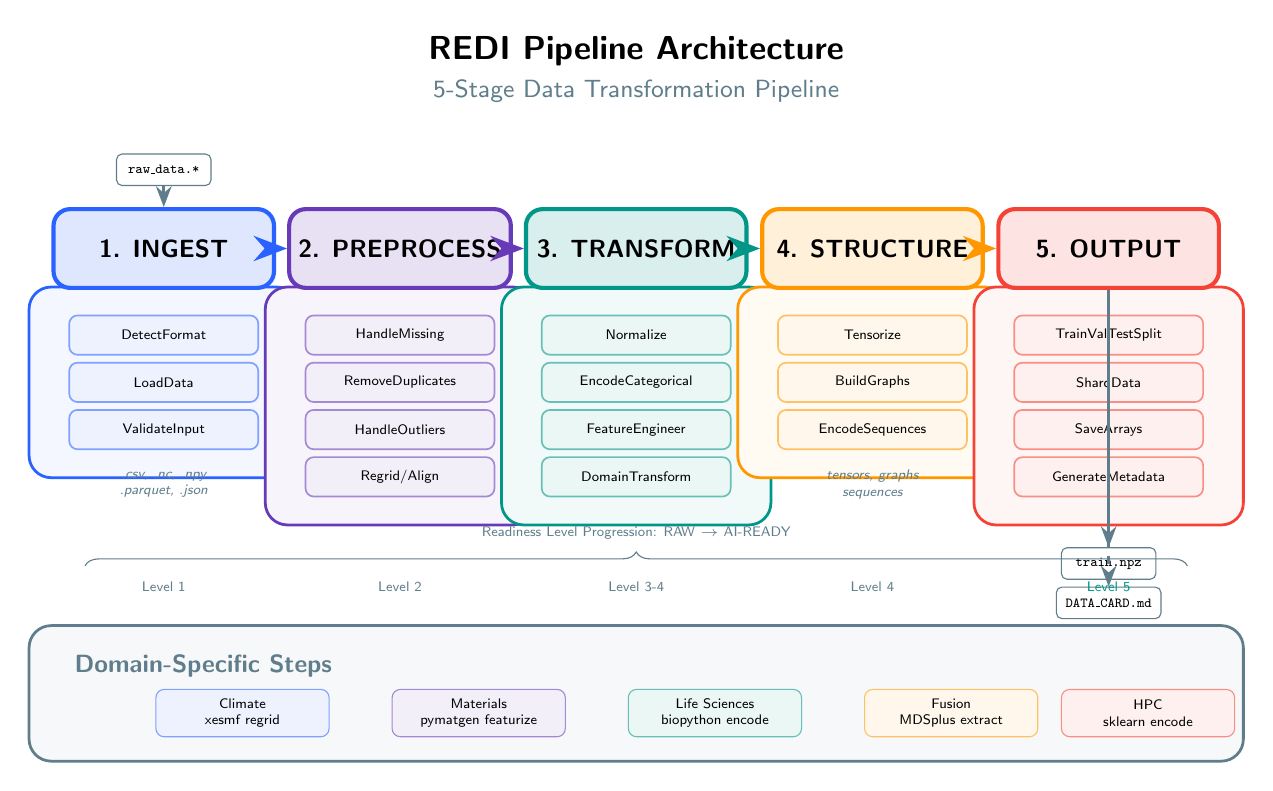
\begin{tikzpicture}[
    stage/.style={
        rectangle, rounded corners=6pt, minimum width=2.8cm, minimum height=1cm,
        draw=#1, line width=1.5pt, fill=#1!15, font=\small\bfseries\sffamily
    },
    step/.style={
        rectangle, rounded corners=3pt, minimum width=2.4cm, minimum height=0.5cm,
        draw=#1!60, line width=0.6pt, fill=#1!8, font=\tiny\sffamily
    },
    file/.style={
        rectangle, rounded corners=2pt, minimum width=1.2cm, minimum height=0.4cm,
        draw=redigray, fill=white, font=\tiny\ttfamily
    },
    arrow/.style={->, >=Stealth, line width=1pt, color=redigray},
    bigarrow/.style={->, >=Stealth, line width=2pt, color=#1},
    groupbox/.style={rectangle, rounded corners=8pt, draw=#1, line width=1pt, fill=#1!5, inner sep=6pt}
]

% Title
\node[font=\large\bfseries\sffamily] at (0, 9) {REDI Pipeline Architecture};
\node[font=\small\sffamily, text=redigray] at (0, 8.5) {5-Stage Data Transformation Pipeline};

% ============================================================================
% Stage 1: INGEST
% ============================================================================
\node[stage=rediblue] (ingest) at (-6, 6.5) {1. INGEST};

\begin{scope}[on background layer]
    \node[groupbox=rediblue, fit={($ (-7.5, 5.8) $) ($ (-4.5, 3.8) $)}] {};
\end{scope}

\node[step=rediblue] at (-6, 5.4) {DetectFormat};
\node[step=rediblue] at (-6, 4.8) {LoadData};
\node[step=rediblue] at (-6, 4.2) {ValidateInput};

\node[font=\tiny\sffamily\itshape, text=redigray, align=center] at (-6, 3.5) {.csv, .nc, .npy\\
.parquet, .json};

% ============================================================================
% Stage 2: PREPROCESS
% ============================================================================
\node[stage=redipurple] (preprocess) at (-3, 6.5) {2. PREPROCESS};

\begin{scope}[on background layer]
    \node[groupbox=redipurple, fit={($ (-4.5, 5.8) $) ($ (-1.5, 3.2) $)}] {};
\end{scope}

\node[step=redipurple] at (-3, 5.4) {HandleMissing};
\node[step=redipurple] at (-3, 4.8) {RemoveDuplicates};
\node[step=redipurple] at (-3, 4.2) {HandleOutliers};
\node[step=redipurple] at (-3, 3.6) {Regrid/Align};

% ============================================================================
% Stage 3: TRANSFORM
% ============================================================================
\node[stage=redigreen] (transform) at (0, 6.5) {3. TRANSFORM};

\begin{scope}[on background layer]
    \node[groupbox=redigreen, fit={($ (-1.5, 5.8) $) ($ (1.5, 3.2) $)}] {};
\end{scope}

\node[step=redigreen] at (0, 5.4) {Normalize};
\node[step=redigreen] at (0, 4.8) {EncodeCategorical};
\node[step=redigreen] at (0, 4.2) {FeatureEngineer};
\node[step=redigreen] at (0, 3.6) {DomainTransform};

% ============================================================================
% Stage 4: STRUCTURE
% ============================================================================
\node[stage=rediorange] (structure) at (3, 6.5) {4. STRUCTURE};

\begin{scope}[on background layer]
    \node[groupbox=rediorange, fit={($ (1.5, 5.8) $) ($ (4.5, 3.8) $)}] {};
\end{scope}

\node[step=rediorange] at (3, 5.4) {Tensorize};
\node[step=rediorange] at (3, 4.8) {BuildGraphs};
\node[step=rediorange] at (3, 4.2) {EncodeSequences};

\node[font=\tiny\sffamily\itshape, text=redigray, align=center] at (3, 3.5) {tensors, graphs\\sequences};

% ============================================================================
% Stage 5: OUTPUT
% ============================================================================
\node[stage=redired] (output) at (6, 6.5) {5. OUTPUT};

\begin{scope}[on background layer]
    \node[groupbox=redired, fit={($ (4.5, 5.8) $) ($ (7.5, 3.2) $)}] {};
\end{scope}

\node[step=redired] at (6, 5.4) {TrainValTestSplit};
\node[step=redired] at (6, 4.8) {ShardData};
\node[step=redired] at (6, 4.2) {SaveArrays};
\node[step=redired] at (6, 3.6) {GenerateMetadata};

% ============================================================================
% Stage Connections
% ============================================================================
\draw[bigarrow=rediblue] (ingest) -- (preprocess);
\draw[bigarrow=redipurple] (preprocess) -- (transform);
\draw[bigarrow=redigreen] (transform) -- (structure);
\draw[bigarrow=rediorange] (structure) -- (output);

% ============================================================================
% Input/Output Files
% ============================================================================
\node[file] (inputfile) at (-6, 7.5) {raw\_data.*};
\node[file] (outputnpz) at (6, 2.5) {train.npz};
\node[file] (outputcard) at (6, 2) {DATA\_CARD.md};

\draw[arrow] (inputfile) -- (ingest);
\draw[arrow] (output) -- (outputnpz);
\draw[arrow, dashed] (output) -- (outputcard);

% ============================================================================
% Domain-Specific Customization
% ============================================================================
\begin{scope}[on background layer]
    \node[groupbox=redigray, fit={($ (-7.5, 1.5) $) ($ (7.5, 0.2) $)}] {};
\end{scope}

\node[font=\small\bfseries\sffamily, text=redigray] at (-5.5, 1.2) {Domain-Specific Steps};

% Domain boxes
\node[rectangle, rounded corners=3pt, draw=rediblue!60, fill=rediblue!8,
      minimum width=2.2cm, minimum height=0.6cm, font=\tiny\sffamily, align=center]
      at (-5, 0.6) {Climate\\xesmf regrid};

\node[rectangle, rounded corners=3pt, draw=redipurple!60, fill=redipurple!8,
      minimum width=2.2cm, minimum height=0.6cm, font=\tiny\sffamily, align=center]
      at (-2, 0.6) {Materials\\pymatgen featurize};

\node[rectangle, rounded corners=3pt, draw=redigreen!60, fill=redigreen!8,
      minimum width=2.2cm, minimum height=0.6cm, font=\tiny\sffamily, align=center]
      at (1, 0.6) {Life Sciences\\biopython encode};

\node[rectangle, rounded corners=3pt, draw=rediorange!60, fill=rediorange!8,
      minimum width=2.2cm, minimum height=0.6cm, font=\tiny\sffamily, align=center]
      at (4, 0.6) {Fusion\\MDSplus extract};

\node[rectangle, rounded corners=3pt, draw=redired!60, fill=redired!8,
      minimum width=2.2cm, minimum height=0.6cm, font=\tiny\sffamily, align=center]
      at (6.5, 0.6) {HPC\\sklearn encode};

% ============================================================================
% Readiness Level Progression
% ============================================================================
\node[font=\tiny\sffamily, text=redigray] at (-6, 2.2) {Level 1};
\node[font=\tiny\sffamily, text=redigray] at (-3, 2.2) {Level 2};
\node[font=\tiny\sffamily, text=redigray] at (0, 2.2) {Level 3-4};
\node[font=\tiny\sffamily, text=redigray] at (3, 2.2) {Level 4};
\node[font=\tiny\sffamily, text=redigreen] at (6, 2.2) {Level 5};

\draw[decorate, decoration={brace, amplitude=5pt, raise=2pt}, color=redigray]
    (-7, 2.4) -- (7, 2.4)
    node[midway, above=8pt, font=\tiny\sffamily, text=redigray] {Readiness Level Progression: RAW $\rightarrow$ AI-READY};

\end{tikzpicture}
\end{document}
